\documentclass[a4paper]{report}
%
% Petidomo Manual
%
% $Header$
%
\usepackage{html}
\usepackage{makeidx}
\usepackage{graphicx}
\makeindex

%
% Self-defined macros
%
\newcommand{\PetidomoM}{{\scshape Peti\-domo Mail\-ing List Ma\-nager}}
\newcommand{\Petidomo}{{\scshape Peti\-domo}}
\newcommand{\PetidomoTwo}{{\scshape Peti\-domo 2.1}}
\newcommand{\Def}[1]{{\index{#1}\sl #1}}
\newcommand{\DefNI}[1]{{\tt #1}}
\newcommand{\file}[1]{{\tt #1}}
\newcommand{\Index}[1]{#1\index{#1}}

%
% Begin of document
%
\begin{document}
\sloppy
\pagestyle{empty}

%
% Titlepage
%
\title{The \PetidomoM}
\author{Peter Simons $<$simons@petidomo.com$>$}
\date{March, 7th 1999}
\maketitle

%
% Copyright
%
\centerline{\huge\bf License Agreement}

\bigskip

\noindent
The "Petidomo Mailing List Manager" is copyrighted \copyright{} 1996--99 by
CyberSolutions GmbH, Germany. All rights are reserved.

\medskip

\noindent
Redistribution and use in source and binary forms, with or without
modification, are permitted provided that the following conditions
are met:

\begin{enumerate}

\item Redistributions of source code must retain the above copyright
   notice, this list of conditions and the following disclaimer.

\item Redistributions in binary form must reproduce the above copyright
   notice, this list of conditions and the following disclaimer in the
   documentation and/or other materials provided with the distribution.

\item All advertising materials mentioning features or use of this software
   must display the following acknowledgement:

     \centerline{This product includes software developed by CyberSolutions GmbH.}

\item The name of the author may not be used to endorse or promote products
   derived from this software without specific prior written permission.

\end{enumerate}

\noindent
You are not required to accept this License, since you have not signed
it. However, nothing else grants you permission to use the program.
These actions are prohibited by law if you do not accept this license.
Therefore, by using the program, you indicate your acceptance of this
license to do so, and all its terms and conditions.

\medskip

\noindent
{\bf This software is provided by CyberSolutions GmbH ``as is'' and
any express or implied warranties, including, but not limited to, the
implied warranties of merchantability and fitness for a particular
purpose are disclaimed. In no event shall CyberSolutions GmbH be
liable for any direct, indirect, incidental, special, exemplary, or
consequential damages (including, but not limited to, procurement of
substitute goods or services; loss of use, data, or profits; or
business interruption) however caused and on any theory of liability,
whether in contract, strict liability, or tort (including negligence
or otherwise) arising in any way out of the use of this software, even
if advised of the possibility of such damage.}

\newpage

%
% Table of contents
%
\pagenumbering{roman} \setcounter{page}{1} \pagestyle{headings}
\tableofcontents
\clearpage
\pagenumbering{arabic} \setcounter{page}{1} \pagestyle{headings}

%
% Begin of actual text
%
\chapter{Quickstart for the impatient}
\index{quickstart}

We know you feel now. You just downloaded the new software
package and are eager to see it work as fast as possible. So, even
though it is kind of mad to write this long manual with the knowledge
that the vast majority of users will never read it, here is a step by
step quickstart guide.

\begin{enumerate}

\item Get the distribution for your Unix platform.

\item Unpack the tar archive: {\tt gunzip <archivename | tar xf -}

\item {\tt su} to the super user.

\item Create a user {\tt petidomo} and a group {\tt petidomo}. The
home directory of this user is the place where the whole package will
be installed. The user doesn't need a valid password and shell.

\item As superuser, {\tt cd} into the directory `petidomo-{\sl
your-architecture-name}' and start {\tt ./install.sh} or {\tt sh
install.sh}.

\item Answer all questions asked by the script truthfully.

\item If no error occurs, send an e-mail to the \PetidomoM: {\tt mail
petidomo </dev/null} and see what happens.

\item Now use your WWW browser to access
\htmladdnormallink{`http://local\-host/cgi-bin/peti\-domo\-conf.cgi'}{http://localhost/cgi-bin/petidomoconf.cgi} and create any mailing
lists you'd like to have.

\item Be happy.

\item Now read the blasted user manual. It was a lot of work to write
it.

\end{enumerate}

\chapter{Introduction}

Congratulations. Obviously you are a clever person. Not only
did you choose the \PetidomoM\ to run your mailing lists, you also
decided to read the user manual. I really appreciate that, mostly
because I strongly dislike writing user manuals and it gives the whole
process at least some sense that someone actually reads it.

For a start, I think, I will bore you with a few historical facts,
which you can absolutely afford to skip if you're in a hurry. What you
probably are. I'll recount the story of \Petidomo\ nonetheless.

\section{History of Petidomo}

Thanks to using version control systems consequently, I was able to
determine that I started working on \Petidomo\ exactly at fourty
minutes after midnight on the December 26th, 1993. I was in desperate
need of a mailing list server for my Amiga computer and so I queried
``archie'' for source codes. (Does anybody remember the days when
``archie'' was still popular?)

What I found was a Unix package called ``Listserv'', which implemented
some basic functionality like subscribing and unsubscribing a mailing
list automatically. Unfortunately there are many differences between
Unix and the AmigaOS, which my computer had. It took until January
9th, 1994 before I had a running version of the program and not even
the small number of commands the Unix version originally had worked.

Anyway, I had my mailing list server and eventually I was able to
release it to the public under the name ``AmigaListserv''. Since it
was the only mailing list server in existance for the Amiga platform,
it became pretty popular after a while and I was flooded with bug
reports, enhancement requests, proposals of marriage and insults of my
general ability to program. So I turned the project into a shareware
product and spent countless hours improving the code and adding new
features. If I remember correctly, I was able to bring two more major
releases out until I had reached ``AmigaListserv version 3.0''.

At some point, though, I became more and more discontend with the
abilities of the Amiga's operating system as an Internet server and at
last I switched to Unix. After looking at various mailing list servers
for the Unix operating system and disliking them thoroughly, I started
porting my own program back to Unix, where it came from originally.

It took quite a while before I had a running version again, but on
December 30th, 1995 ``Listserv 4.0 beta'' took over my mailing lists on
Unix. Needless to say that porting a souce code between two different
systems twice leaves traces behind. The source code was a mess and the
number of recursive defines, redefining what other defines had been
redefined before had increased beyond the point where you call a
source code ``spaghetti code''.

Nonetheless, around May 1996 I faithfully release the 1.0 version to
the public under GNU General Public License and waited for feedback.
The first mail that arrived after my announcement in the USENET-news
was a mail from an L-Soft employee who told me that I would be sued if
I wouldn't change the name of my package, because they were selling a
program called ``LISTSERV'' for years already and had protected the
name.

So I renamed my package to ``\Petidomo\ 1.0'' and released it again.

The number of installations \Petidomo\ quickly had, and the number of
positive feedback I received exceeded my expectations by far. Clearly,
I must have been doing something right, if a serious number of people
preferred my package over the way more powerful alternatives for Unix,
like Majordomo, Smartlist, Procmail and LISTSERV.

Again I started improving the functionality, cleaning up the code,
making it more portable and stable and so on\dots{} \Petidomo\ reached
release number 1.3 on December 27th, 1996, almost exactly three years
after I started working on the very first version.

\Petidomo\ 1.3 was a widely used and appreciated package, it was stable,
very portable, easy to understand and to maintain and it was all in
all pretty neat. So I deleted all the source codes and started
re-writing it from the scratch.

Don't ask why, programmers do these things occasionally.

The result of this effort is \PetidomoTwo, as you can see. The 2.1
version exceeds \Petidomo\ 1.x's functionality and power in absolutely
every aspect, while being even easier to setup and to maintain. Not a
single line of code from the original 1.x version was used and the
benefit of this is a very modern and efficient design that I am quite
proud of.

Some people are disappointed that the 2.1 version is a commercial
product now, but too much time and effort has been put into it to give
it away for free, I am afraid. But I think the ``free for
non-commercial use'' clause is fair for everybody.

Well, thanks for bearing with me during all this gossip, but I felt
obligated to tell this story.

And now have fun with the technical part of the manual and I hope you
like my program.

\section{Acknowledgments}

Many people contributed to the development of \Petidomo\ directly or
indirectly, and we would like to thank everybody for their help at
this point.

Hey, all you beta testers: This paragraph is for you. I bet you still
can't believe that there's an actual manual for \Petidomo\ available
now. Be assured of our deep respect and gratitude for managing to use
a software package that was sometimes unstable and weird, and always
undocumented except for a totally outdated README file.

A big ``thank you'' to Markus Fleck of the University of Bonn for
providing us with an FTP mirror of the \Petidomo\ Beta distributions.

Furthermore, our appreciation to Gray Watson for writing the excellent
``argv'' and ``dmalloc''-libraries, which have been used in the
\PetidomoM\ during the beta testing phase.

And last, but not least, the developers would like to thank the team
of CyberSolutions~GmbH for their support during the development,
for taking over all the marketing stuff while we were programming and
for providing the Internet WWW server for \Petidomo.

\chapter{What is a mailing list anyway?}

This chapter is meant as an introduction into the principles of
mailing lists, the way a mailing list server works and the terminology
commonly used in this context. For the beginner, it is recommended to
read this chapter carefully, as many of the terms used in the rest of
the manual will be explained here. Advanced readers can safely skip
this chapter because it does not describe the \Petidomo\ mailing list
server in particular and is not relevant for configuring and using the
package.

\bigskip

Electronic mail is still the most-used service in the Internet, and
not the WWW, as one might expect. It use it for causual conversations
between people all over the world, for discussions of all kind of
topics, for transmitting data files through the net or for
distributing information amongst colleagues in a world-wide company.
Even in Intranets electronic mail is very useful, because it is quick,
easy to archive and reliable.

Electronic mail is not limited to conversations between only two
peers. A mail may have several recipients unlike a paper letter.
Hence, discussions between groups of people can be held with this
media easily. Everybody sends the mail to all persons involved in the
discussion and everybody can reply in a way that all others see his
text, too.

For larger groups of people, though, this becomes inconvenient. When
exchanging e-mail in a larger group of recipients, people tend to
accidently forget persons in the list of recipients, they send their
replies to the wrong person, they have to keep their aliases
up-to-date for the mail to reach the person, etc\dots{}

To remedy these shortcomings, the idea of the mailing list was
developed. A mailing list is \DefNI(hosted)\index{hosting a mailing
list} on a central server, which has the addresses of the people who
are on that mailing list. Then a special account is created, called
the \Def{mailing list address}, to which people can send the mail they
want to be distributed to all receivers.

\begin{figure}[bth]
\begin{center}
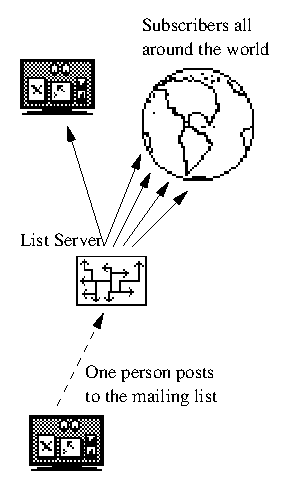
\includegraphics{ml-principle1.eps}
\caption{A mail is posted to the mailing list.}
\end{center}
\end{figure}

The machine accepts the mail, looks up the list of addresses in the
list, and re-sends the mail to all those people. If one of the persons
on the list wants to reply to a mail he or she has received via the
mailing list, he or she sends the reply to the mailing list address
again and it is automatically distributed among all recipients again.

The list of addresses on the machine hosting the mailing list is
called the \Def{list of subscribers} and a person who is on that list
is consequently called a \Def{mailing list subscriber}. The process of
sending an e-mail to the special address with the intention to get it
distributed to all subscribers is called \Def{posting to a list}.

\begin{figure}[bth]
\begin{center}
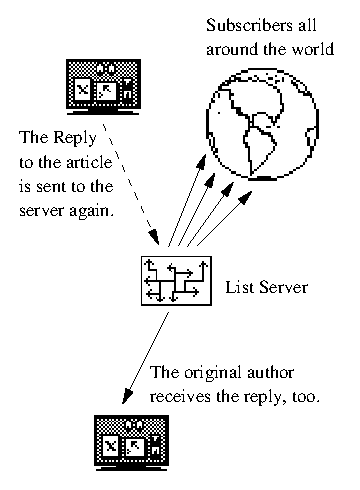
\includegraphics{ml-principle2.eps}
\caption{A subscriber replies to the mail.}
\end{center}
\end{figure}

The advantage of this setup is that each subscriber only has to know
the address of the mailing list and not all the addresses of all the
subscribers. In fact, a subscriber doesn't even have to know who is
subscribed to the mailing list at all.

Imagine the company you're working for would have a mailing list where
all employees are subscribed with their current e-mail address. The
mailing list address would then be, say,
``all-employees@enterprise.com''. If you'd like to inform all your
colleagues about an important happening, you'd simply send an e-mail
to that address and everybody would receive it. If a person leaves the
company, or a new employee comes to the company, only the list of
subscribers on the mailing list server has to be updated and
everything would work fine.

Basically, this is what a mailing list server does: It is nothing more
than a program that stores a list of addresses, receives mail under a
special mailing list address and then re-sends the mail to all
subscribers.

Of course you're not limited to one mailing list, you can host as many
as you like. Not only a list for all employees, but also discussion
forums for the management of the company, for all members of a certain
department or all the left-handers. Privately, you can use mailing
lists to discuss your favourite hobby with other interested people,
you can spread basketball statistics or the latest version of a
program all the subscribers are using. There's no limitation. Whenever
a group of people has to exchange electronic mail on a regular basis,
a mailing list is a good way to do it.

\bigskip

As you can probably imagine, the task of keeping the list of
subscribers up-to-date becomes a bit difficult when the number of
subscribe addresses grows beyond a few dozen, because people tend to
change their e-mail addresses from time to time, for various reasons.
On a mailing list for a thousand subscribers from all over the world,
the maintainer of the list would probably spend most of his time
editing the list file, removing or adding addresses.

That is why \Petidomo\ allows people to do that themselves.
Additionally to the part that re-sends the mail to all subscribers,
there's a program included in the package that understands a number of
commands, like ``subscribe'' or ``unsubscribe''.

If you want to have your address added to a mailing list, you do not
contact the maintainer of the list, but you send an e-mail to
\Petidomo\ and put the command ``subscribe'' into the mail. \Petidomo\
will then add your address to the list automatically. Not only is this
easier and more convenient for you, it is also a lot faster. Usually,
\Petidomo\ will process a subscription request for a mailing list in a
tenth of a second, 24 hours a day, while a human maintainer of the
list would probably need several hours or even days to cope with the
incoming e-mail.

Similarly you can remove your address from a mailing list, or you can
change the address you are subscribed under within a few moments and
now human interaction is required.

So how does this work? It's very easy in fact: The command interpreter
of the mailing list server has a special address, too. This is the
name of the list, with the text ``-request'' append to it. All e-mails
directed to this account will be processed by the server. If, for
example, you want to subscribe to a mailing list with the name
``basketball'', which has the address ``basketball@nba.com'', you'd
send an e-mail to the address ``basketball-request@nba.com'' and put
the word ``subscribe'' in the body of the mail.

\Petidomo\ would then receive the mail a few moments later, process
it, add your address to the list of subscribers and send you a short
recipt back to let you know that your subscription was successful.

It is very important that you know the difference between the address
of the mailing list itself, and the program that is maintaining the
list of addresses. If you'd write your mail to ``basketball@nba.com''
--- to stick with our example --- instead of
``basketball-request@nba.com'', your command would not be processed by
the server but would be re-sent to all subscribers. This is a common
mistake beginners make and it is a particular annoying one, because
the subscribers are bothered with the useless article on the list, and
secondly, because the person who tried to subscribe will not get what
he or she wanted: To be subscribed to the list.

The type of mailing list we have described so far is known as a
\Def{public mailing list}. That is a list that is open to everyone to
subscribe. Opposed to that is a \Def{closed mailing list}. That is a
mailing list where only certain people may subscribe or where every
subscription requests needs the approval of the list maintainer to
succeed.

The public mailing list is widely used in the Internet for all kind
discussion forums, while a closed mailing list is typically used by
companies or organizations for maintaining internal forums, that are
not meant for everybody. \Petidomo\ can maintain both kind of lists,
of course, and a number of variations between the public and the
closed list, so it will usually suit your needs just fine.

\chapter{Installing Petidomo}

The installation of the \PetidomoM\ is mostly handled by the script
\file{install.sh}, which is included in the distribution. But before
the script can be run, a few preperations have to be done manually.

Just follow the steps as described below:

\begin{enumerate}

\item Become `root'. You will need super user privileges.

\item Create a user \index{petidomo-user} `petidomo' using vipw(8),
     adduser(8) or whatever method your system uses. The user should
     not have a valid shell, nor a valid password because it is very
     unlikely that anybody ever needs to log in as `petidomo'. The
     home directory, though, is of some importance because the
     directory you specify here is the base directory for the whole
     \Petidomo\ installation. An example entry in \file{/etc/passwd}
     looks like this:

\begin{verbatim}
     petidomo:*:300:300:Petidomo Mailing List Manager:
         /usr/local/petidomo:/usr/bin/true
\end{verbatim}

     This means that all files belonging to \PetidomoTwo\ live in the
     \file{/usr/lo\-cal/pe\-ti\-domo} tree. The entry in the password file can be
     changed at any time. Hence it is very easy to move \Petidomo\
     \index{Moving Petidomo} to a different location or to de-install
     the whole package.

\item Create a group `petidomo' and make the `petidomo'-user a member of it.
     You should also add all users of your system, that will administrate
     the mailing list server. Membership in the `petidomo' group will give
     these users full access to all configuration files, so be careful who
     to add.

\item index{install.sh} \index{Install script} As `root', execute the
     install script included in the distribution with `./install.sh'
     The script will ask you a couple of questions about your system
     and insert the appropriate values in the config files. Ones the
     script is finished, your \Petidomo-Installation is complete and
     ready to run.

\end{enumerate}

If choose not to let the install script create the required aliases
for \Petidomo, you will have to do that manually as described in
section~\ref{aliases} of the manual.

\section{Logfiles}

Reading the log files \Petidomo\ writes the single most important
thing you have to do whenever something unexpected happens. Often
enough the problem is very easy to to fix, if you know what the
problem actually is. To support you in locating problems, \Petidomo\
does extensive logging, espcially in case of an error.

For this, \Petidomo\ uses the syslog(3) functionality, which is part
of every major Unix derivate today. \Petidomo\ uses the {\tt
MAIL}-facility to log via syslog, so it is recommended, that you check
your \file{/etc/syslog.conf} file, whether you are writing the {\tt
MAIL}-facility into a file or not. Typically an entry in
\file{/etc/syslog.conf} would look like this:
\begin{verbatim}
mail.*                           /var/log/maillog
\end{verbatim}

If you are unfamiliar with the syslog-functionality, please read the
following man pages: syslog.conf(5), syslogd(8) and syslog(3). They
explain all the features briefly and you will greatly benefit from the
knowlege --- not only for using \Petidomo, but for maintaining your
whole system.

\section{Directory Structure}

\begin{figure}[bth]
\begin{center}
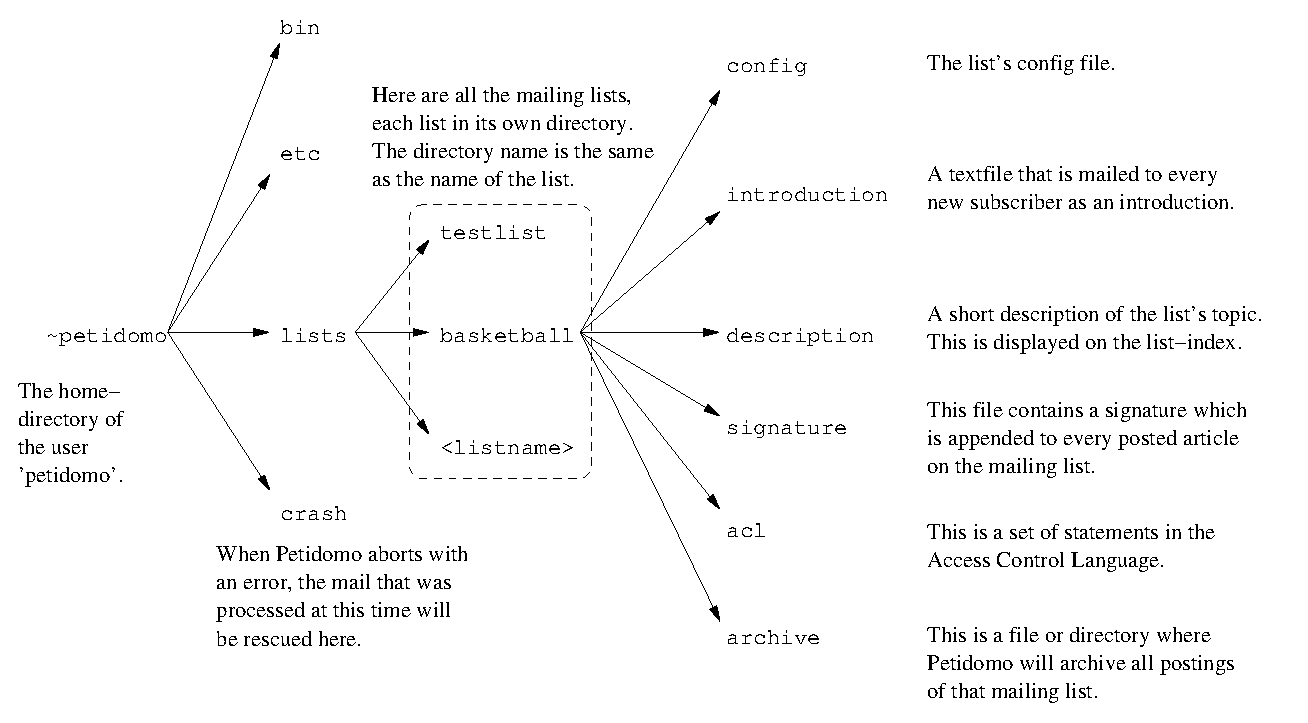
\includegraphics[width=\textwidth]{directory-struct.eps}
\caption{The \Petidomo\ directory structure.}
\label{directory structure}
\end{center}
\end{figure}

Before we dive into the details configuration of \Petidomo, it is
necessary to describe the \Index{directory structure} of the package.
\Petidomo's base path, which we call \Def{\~{}petidomo} throughout the
manual, is the home directory of the `petidomo' user. Relative to this
directory, \Petidomo\ accesses its master config file as
\file{etc/petidomo.conf}. This is the so called \Def{master config
file}, which sets globally required options such as the path to the
mail transport agent (MTA), the fully qualified domain name of the
machine, \Petidomo\ is running on, etc\dots{}

Each list now has a config file of its own, where various settings are
configured that are valid only for that list locally. All mailing
lists live in the path \file{lists/$<$listname$>$}, with ``$<$listname$>$''
being the name of the mailing list. The config file for the mailing
list ``testlist'' can congruously be found under the path
\file{lists/testlist/config}, relative to the base directory of
course.

\section{The Config-Files}

We will describe the master config file first now, followed by the
options you can set on a per-list basis. You won't have to edit all
these files yourself. The CGI manager, which is described in detail in
section~\ref{using the cgi manager}, is usually a more comfortable way
of configuring \Petidomo. You should read the following description
nonetheless, because you need to know what an option \emph{means},
even if you don't have to set it with a text editor.

\subsection{Config File Syntax}

All configuration files in the \Petidomo-package\index{Config file
format}\label{Config file format}, have the following format:
\begin{verbatim}
keyword         parameter
\end{verbatim}

The ``keyword''-part must start at the first column of the line and is
followed by one or several blanks or tabs. The first non-blank
character then is interpreted as the parameter for this keyword. The
following line, for example:
\begin{verbatim}
Hostname        petidomo.is.great
\end{verbatim}
will tell \Petidomo\ that the name of the machine it is running on is
called ``petidomo.is.great''. If the parameter contains any blanks,
what is not very likely for a hostname, but may happen with other
settings, you should enclose it in double quotes, like this:
\begin{verbatim}
AdminPassword   "open sesame"
\end{verbatim}

Quoting the parameter is not strictly necessary, though, \Petidomo's
config file parser will get it right anyway. You only have to quote
the parameter, if it contains blanks as first or last character, what
is rather unlikely to happen. If you're using the CGI manager for the
configuration, you won't have to worry about quoting at all.

Furthermore all empty lines are ignored. So are lines that start with
a `\#' sign. You can use this for writing comments for the reader into
the config file.

\subsection{The Master Config File}
\label{master config file}

\Petidomo\ expects its master config file to be found under
\file{\~{}peti\-do\-mo/etc/pe\-ti\-domo.conf}. The following keywords are
recognized:


\begin{description}

\item[Hostname] \hfill ``hostname.domainname''
\index{Hostname}

This entry specifies the fully qualified domain name of the machine,
\Petidomo\ is running on. A \Index{fully qualified domain name} is the
hostname of the machine with the domain name appended with a dot. The
following, for example:
\begin{verbatim}
HostName        listserver.foo.bar
\end{verbatim}
would be a valid statement. Normally this option has been set by the
install script correctly already.

The name you set here is not necessarily the name, \Petidomo\ will use
when delivering mailing list-postings to the subscribers, or when
answering requests, because you can specify a different fully
qualified domain name for every mailing list you host. This is known
as \Def{virtual hosting}.

This option is \emph{required}. \Petidomo\ will abort with an error,
if the master config file doesn't set it.

\item[AdminPassword] \hfill ``password''
\index{AdminPassword}

This tag sets the master password, which authenticiates the
administrator of the \PetidomoM. Here is an example:
\begin{verbatim}
AdminPassword   "open sesame"
\end{verbatim}
Normally this option has been set by the install script already.

Please chose this password carefully. Knowledge of the master password
will enable you to access \emph{all} mailing lists running on this
system.

The password comparison both \Petidomo\ and the CGI manager do, are
always case insensitiv. That means, that the passwords ``Open
SESAME'', ``open sesame'' and ``OPEN seSAme'' are all the same.

This option is \emph{required}. \Petidomo\ will abort with an error,
if the master config file doesn't set it.


\item[MTA] \hfill \file{/path/to/sendmail}
\index{MTA}\index{mail transport agent}

The MTA tag tells \Petidomo\ which mail transport agent should be used
to deliver outgoing emails. Normally this option has been set by the
install script already, so you don't need to worry about this anymore.

An example setting is:
\begin{verbatim}
MTA     "/usr/sbin/sendmail"
\end{verbatim}
but \Petidomo\ will run fine with other mail transport agents, too. So
far, the system has been tested with the Allman sendmail, SMail and
qmail without any problems.

This option is \emph{required}. \Petidomo\ will abort with an error,
if the master config file doesn't set it.


\item[MTA\_Options] \hfill ``string''
\index{MTA\_Options}

This tag is a bit tricky and in ninety-nine out of hundred cases you
should simply leave this option undefined as it is rarely required
anyway.

This entry sets the options which will be handed over to the MTA
when it is called. The following example
\begin{verbatim}
MTA_Options "-odq -v -f%s"
\end{verbatim}
will yield a call ``$<$MTA$>$ -odq -v -f$<$envelope$>$''. The `\%s' is
replaced with the envelope the mail should be sent under.

Adding options to the execution call of the mail transport agent can
be useful to enable or disable certain features for mailing lists
only, while leaving them on for all other mail. The `-odq' setting is
a fine example. This parameter will tell the Allmann sendmail to queue
all mail, instead of trying to deliver it immediately.

\item[DetachImmediately] \hfill ``yes'' or ``no''
\index{DetachImmediately}

This option decides whether \Petidomo\ will run in syncronous or
asyncronous mode. When a part of the package is called, it expects an
incoming email message on standard input, which has usually been
received by the SMTP daemon before. So the daemon will pipe the mail
into the program.

In syncronous mode, \Petidomo\ will process the mail completely, before
it terminates. Hence, the SMTP daemon has to wait until the whole mail
is processed, before it can terminate itself. This may cause memory
problems at high-load servers, where several dozen, or even hundreds
of emails can arrive at the same time.

In asyncronous mode, \Petidomo\ will read the mail and then detach
itself. The advantage is that the SMTP daemon can terminate
immediately and doesn't have to wait until \Petidomo\ is finished
processing the mail. The disadvantage is that in case of an error, the
SMTP daemon will not receive the return code from \Petidomo. For
smaller servers, syncronous mode is recommended --- larger servers
should use asyncronous mode.

To run in syncronous mode, set the parameter to ``no'':
\begin{verbatim}
DetachImmediately       no
\end{verbatim}
to run in asyncronous mode, set the parameter to ``yes'':
\begin{verbatim}
DetachImmediately       yes
\end{verbatim}

The default, if the option is unset, is to operate syncronously.

\item[ShowStatistics] \hfill ``yes'' or ``no''
\index{ShowStatistics}

\Petidomo\ will append a small signature to all request-mails it
processes. This signature looks like this:

\begin{quote}
\begin{verbatim}
--
 /*
  * Listserver software: Petidomo 2.2-beta-2 (non-commercial)
  * Server hardware    : NetBSD-i386
  * Utilized cpu time  : 0.125863 seconds
  * Utilized memory    : 227 KByte
  */
\end{verbatim}
\end{quote}

You can switch this behavior off by setting this option to ``no''.

\end{description}

\subsection{The list config file}
\label{list config file}

While the master config file sets options which are relevant for the
\Petidomo\ package as a whole, the \Index{list config file} sets
options which are valid only locally for the mailing list. Each
mailing list expects its local config file to be found at
\file{\~{}petidomo/lists/<listname>/config}, with ``$<$listname$>$''
being the name of the mailing list.

For a description of the config file format, please refer to
section~\ref{Config file format} of the user manual. We will only
describe the various settings here.

\begin{description}

\item[ListType] \hfill ``open'', ``closed'' or ``moderated''
\index{ListType}

There are three types of mailing lists \Petidomo\ knows about: ``Open
lists'' (or ``public lists''), ``closed lists'' and ``moderated
lists''. The difference betweem the three types is, who is allowd to
post an article on the mailing list.

If you want everybody to be able to post to the mailing list, whether
he is subscribed or not, you should set this entry like this:
\begin{verbatim}
ListType        open
\end{verbatim}

If you want to allow only postings from people, who are subscribed to
the list, set the entry as follows instead:
\begin{verbatim}
ListType        closed
\end{verbatim}

Or, if you want to allow only a small number of people to post, set
the list to ``moderated'':
\begin{verbatim}
ListType        moderated
\end{verbatim}

Please note that the ``ListType'' tag specifies only who is allowed to
\emph{post}, not who is allowed to subscribe to the list.

The list type you will usually use is ``open'', at least for a public
mailing list where everybody is free to subscribe. The ``closed'' list
has been added, because open mailing lists are frequently abused by a
few people who use them to distribute commercial advertisement.
Because these people (common known as \Def{Spammer}s) do not actually
subscribe to the list, but merely post their junk to it, their abuse
will be rejected on a closed forum, while all the regular users can
post without any problems.

The problem is, though, that the distinction between a subscriber and
a non-subscriber is made by the address the e-mail is coming from.
This causes problems when a person is subscribed to a list as
``example@address.net'', but tries to post from a different account
than that one. \Petidomo\ tries to recognize that as far as it can.
It doesn't matter, for example, whether you are posting from
``address@host1.address.net'' or ``address@host2.address.net''.
\Petidomo\ will handle that. But if the article comes from
``example@private.account'', it will be rejected, even though the
sender might be a valid subscriber.

It depends on the subscribers of the mailing list, whether this is a
problem or not.

A moderated list, finally, is a list where all postings will be
rejected unless they have a valid password included in the mail. This
type of list is useful for a mailing list that is meant to distribute
certain information to a group of people, but not for discussion.
Everybody, who wants to have an article delivered to the subscribers,
will send it to the mailing list. The list server will then forward
the article to the list maintainer for approval.

The list maintainer can now either drop the mail, if it doesn't fit
into the list's topic, or he can post it to the list, using the
propper password. How this is done in detail is exlained in
section~\ref{petidomo as admin} of the user manual.

This option is \emph{required}. \Petidomo\ will abort with an error,
if the list config file doesn't set it.

\item[AllowPublicSubscription] \hfill ``yes'' or ``no''
\index{AllowPublicSubscription}

Set this entry to either ``yes'' or ``no'', depending on whether you
want the mailing list to be open for everybody to subscribe or not.

If somebody tries to subscribe to a mailing list, which has been set
to ``no'' here, the request will be forwarded to the list
administrator for approval by \Petidomo.

If this option is unset, the default to allow public subscription.

\item[AllowAlienSubscription] \hfill ``yes'' or ``no''
\index{AllowAlienSubscription}

Please excuse the name of this tag, but no matter how hard we thought,
we were unable to come up with a better name for it. If you have any
suggestions, please send them to $<$simons@petidomo.com$>$.

Anyway, this option specifies whether it is allowed to subscribe or to
unsubscribe an address not equal to the one, the mail has been sent
from. Set the option to ``yes'' to allow un-/subscribing a different
address, or to ``no'' to disallow it.

\item[AllowMembersCommand] \hfill ``yes'' or ``no''
\index{AllowMembersCommand}

\Petidomo\ knows a command ``members'' or ``who'', which can be sent
to the server and it will reply with the complete list of subscribed
addresses for the mailing list. This may be useful for list
administrators, but it can be abused easily by spammers, to collect
addresses where to send their unsolicted commercial e-mail to.

Furthermore, with certain mailing lists it may be undesirable that one
can see ``who else'' is subscribed to that list. That's why this
option has been added. If you set it to ``no'', the
``members''-command will be diabled for this list. (This is also the
default if the option is not specified in the config file.)

If you set it to ``yes'', the ``members''-comman will work.

\item[ShowOnIndex]  \hfill ``yes'' or ``no''
\index{ShowOnIndex}

\Petidomo\ allows people to request a list of mailing list running on
the server, using the ``index'' command. While it is generally a good
thing that everybody can look up what mailing lists exist, there are
mailing lists that you don't want to make publically known, such as
internal lists of your company, etc\dots{}

If you set this option to ``no'', the mailing list will not appear on
the index listing. The default, if this option is unset, though, is
``yes'' --- to show the mailing list.


\item[Hostname] \hfill ``hostname.domainname''

This options tells \Petidomo\ to use this hostname for the mailing
list, instead of the one configured in
\file{\~{}petidomo/etc/petidomo.conf}. This feature is useful to do
virtual hosting.

\DefNI{Virtual hosting}\index{virtual hosting} is required when
several mailing lists run on the same server, but they have to look
like they would coming from different machines. Let's use an example:
The internet service provider ``Inter.Net'' offers its customers to
host mailing lists for them. A small software house of the name
``Petiware'' wants to provide a mailing list for all its customers,
but they don't have a dedicated Internet line.

So they use the service provided by Inter.Net and let them host the
mailing list on their machine. The mailing list server at Inter.Net
has the fully qualified domain name ``mail.inter.net''. Petiware,
though, wants the list to run under the name
``customers@petiware.com'' and \emph{not} ``customers@inter.net'' ---
what would a be misleading.

So all the mailing list guru from Inter.Net has to do is to set the
entry
\begin{verbatim}
Hostname        petiware.com
\end{verbatim}
in the config file of the ``customers'' mailing list
(\file{\~{}peti\-domo/lists/cu\-stomers/config}). \Petidomo\ will now use the
hostname ``peti\-ware.com'' in all mails that are posted to that list,
instead of ``mail.inter.net''.

You can specify a different hostname for every mailing list, using
this feature. \emph{That} is ``virtual hosting''. Further details on
virtual hosting can be found in section~\ref{virtual hosting and
sendmail} of the user manual.

If this entry is unset, the name configured in the master config file
will be used as hostname for this mailing list.

\item[AdminPassword] \hfill ``password''
\index{AdminPassword}\label{list admin password}

This tag sets the master password, which authenticiates the
administrator of this mailing list. The administrator has special
priviledes, such as deleting other users, overriding access control
restrictions or un-/subscribing users to closed mailing lists. This is
described briefly in section~\ref{petidomo as admin} of the user manual.

Please note that passwords are always case-insensitive. It is also
worth noting that the master password is always valid as administrator
password for the list, also.

Leave this entry blank, if you don't want to enable remote
administration of the mailing list.

\item[PostingPassword] \hfill ``password''
\index{PostingPassword}\label{posting password}

This tag sets the ``posting password''. The posting password allows to
post an article to a moderated mailing list, but it does not allow any
administration of the list itself. On lists that are of a different
type than moderated, setting a posting password does usually not make
any sense and you can leave this entry unset.

\item[ReplyTo] \hfill ``email@address.net'' or ``none''

This tag controls the `Reply-To:' field, which \Petidomo\ adds to
posted articles before it is delivered to the recipients. Using this
option, you can force \Petidomo\ to insert a `Reply-To:' which points
to a certain address. On a moderated list, for example, you can set
this as follows:
\begin{verbatim}
ReplyTo         moderator@address.net
\end{verbatim}
to direct all replies to the posting to the moderator again,
regardless of what address is noted in the `From:' line of the mail.

If you set ``none'', \Petidomo\ will not add a `Reply-To:' header at
all.

If this option is unset, \Petidomo\ will to insert a `Reply-To:'
header that directs replies back to the mailing list, so that
subscribers can conveniently post simply by hitting the `reply'
function in their mail reader.

\item[PostingFilter] \hfill ``bourne shell command''
\index{PostingFilter}

If you specify a posting filter, this program or script will be
started by \Petidomo\ before it sends a posting out to the
subscribers. The programm will receive the article, as it has been
prepared by Petidomo, on standard input and is expected to write the
final version of the mail to standard output. The posting filter can
be used to manipulate the headers for special purposes.

An example for a postin filter that wouldn't modify the mail at all is
the following:
\begin{verbatim}
PostingFilter   /bin/cat
\end{verbatim}

A detailed discussion of posting filters can be found in
section~\ref{using posting filters} of the manual.

If the filter program exits with a returncode not equal to 0 (zero),
\Petidomo\ will not post the article and terminate.


\item[Archive] \hfill \file{/path/of/archive}

If this option is set, \Petidomo\ will archive all articles that have
been posted on that mailing list. The parameter for this tag may
either be the name and path of a file or of a directory.

The path may either be absolute (\file{/var/archive/list}) or relative
(\file{archive}). For relative paths the current directory is the home
directory of the mailing list this option is set for.

If the ``Archive''-tag is set to a file, \Petidomo\ will append every
posted article to that file. If it is a directory, each posting will
be stored in that directory in a seperate file.

Creating a mailing list archive is discussed in greater deatil in the
section~\ref{mailing list archives} of the user manual.

If this option is unset, posted articles will not be archived at all.

\end{description}

\section{The CGI Manager}

\Petidomo\ comes with a CGI program, that lets you do all the
configuration out of your favourite WWW-Browser. This program is
called \Def{petidomoconf.cgi} and it is installed by the
install-script into the \file{cgi-bin} directory of your HTTP daemon
--- unless you skipped that part, of course.

\subsection{Installing the CGI Manager}

If you did, you can still ``install'' the CGI manager simply by
copying the \file{petidomoconf.cgi} binary from
\file{\~{}petidomo/bin/petidomoconf.cgi} into the appropriate directory.
The binary should be owned by `root:petidomo' and be installed with
the ``setuid'' and ``setguid'' flag set. You can do this by executing
the commands
\begin{verbatim}
$ chown root petidomoconf.cgi
$ chgrp petidomo petidomoconf.cgi
$ chmod 6555 petidomoconf.cgi
\end{verbatim}

Superuser privileges are required only when creating or removing a
mailing list with the CGI manager. In all other cases, the program
will give up the super user privileges immediately, to reduce the
chance of any abuse.

If you don't want to grant `root'-access to the CGI manager, you
should install it with the `petidomo'-user as owner and still set the
`setuid' and `setguid' flags. If you're creating a mailing list in
such a setup, you will have to add the appropriate aliases manually,
though. How this is done is explained in section~\ref{aliases} of the
manual.

The only way around this is to make the \file{/etc/aliases} file
writable for the user or group `petidomo'. Then the CGI manager will
be able to access the file without `root' privileges.

It is recommended, though, to grant `root'-privileges to the CGI
manager as this makes the administration of your mailing list server a
great deal easier.

It should be noted that the CGI manager will run the ``newaliases''
command after you have created a new mailing lists, or removed an
existing list with it, because these operations change the alias file
and sendmail won't notive that until ``newaliases'' is run. For this
to succeed, you must have this program into the execution path of your
shell, because the CGI manager doesn't know about the full path where
``newaliases'' is. On all systems we used to test this, the CGI
manager ran ``newaliases'' successfully, so you probably shouldn't
worry about this.

But if you notice that the changes made with the CGI manager don't
take effect immediately, you should either fix the {\tt \$PATH}
variable on your system, or copy the ``newaliases'' into a directory,
where the CGI manager can find it, for example \file{/usr/bin}.

\subsection{Using the CGI manager}
\label{using the cgi manager}\index{CGI Manager}

\begin{figure}[bth]
\begin{center}
\includegraphics{cgi-manager1.ps}
\caption{The CGI manager login screen.}
\label{cgiman login}
\end{center}
\end{figure}

The CGI manager is rather easy to use. Once it is propperly installed
in the \file{cgi-bin} directory of your WWW server, you can access it
under the URL:
``\htmladdnormallink{http://localhost/cgi-bin/petidomoconf.cgi}{http://localhost/cgi-bin/petidomoconf.cgi}''.
Please note that the CGI manager \emph{must} be installed on the same
machine as the mailing list server. It has to modify the config files
on the harddisk and obviously can't succeed when it is running on a
different machine, say, a dedicated web server.

If you access the CGI manager from your WWW browser, you'll see the
login screen, as shown in figure~\ref{cgiman login}. The CGI manager
prompts you for the password to authenticate yourself. Please enter
the password, you specified to the install-script now, choose the
``Configure Petidomo 2.1'' button and click on ``Submit Query''.

Your WWW browser will now present you a page with several text fields,
where you can enter the parameters you'd like to set. If you change
and submit the changes, they will be written back to the master config
file in \file{\~{}petidomo/etc/petidomo.conf}. The meaning of the
parameters here is the same as described in section~\ref{master config
file}.

If you choose ``Configure an existing mailing list'', the CGI manager
will present you a list of lists it has found. Select the list you''d
like to configure and hit ``Submit Query'' to enter the actual
configuration page.

It should be noted that you will only see the mailing lists, that you
password is valid for. If you entered the master password, which is
configured in the master config file, you will have access to all
mailing lists running on the machine. It is possible, though, to set
an admin password (see section~\ref{list admin password}) for a
mailing list, too. If you entered this password, instead of the master
password, you'd see only this particular list at the moment. In case
several mailing lists have the same admin password, you'll see all of
them.

This behavior is very useful if you are hosting mailing lists that are
administrated by other people. Just tell the administrator of the hosted
mailing lists ``their'' password and the URL of the CGI manager, and
thez will be able to configure ``their'' mailing lists
remotely\index{remote configuration} without gaining access to the
other mailing lists running on the server.

Anyway, select the ``testlist'' entry now and enter the configuration.
As before, a page will be shown where you can customize all the
options that have been described in the section~\ref{list config file}
of the manual. The changes you make will then be written back into the
list's config file. In our example, this would be
\file{\~{}petidomo/lists/testlist/config}.

The remaining two choices on the main page of the CGI manager are
``Create a new mailing list'' and ``Remove an existing mailing list''.
These two should be pretty self-explanatory. If you chose to remove a
mailing list, you will be prompted for the list you'd like to remove
and by submitting the selection, it will be deleted from the server.

Creating a new mailing list works exactly like configuring a new
mailing list except for the fact you'll notice four additional text
fields at the top of the page, compared to the configuration page. The
first text field is for entering the name of the mailing list.
\index{mailing list names} You must choose a list name, that doesn't
contain any special characters, like the slash ('/'), the colon (':')
or the point ('.'), as these have special meanings to either the file
system or to the mail transport agent. The best is to stick with
normal characters and numbers, plus the minus (`-'), for example:
``basketball-fans'' or ``petidomo-support''.

In the second text field, you should enter a short \Index{description}
of the purpose and topic of the mailing list. This text is displayed
when a user requests the index of available mailing lists from the
server and it can be requested by sending the command ``HELP
listname'' to the list server. For our example mailing list
``basketball-fans'', a good description would probably be:

\begin{quotation}

This mailing list is a public forum meant for discussion of the topic
of ``basketball'' or all related topics. This is not a fan list for a
particular basketball team or player, but a forum for all fans of the
sport basketball.

\end{quotation}

A similar function has the third text field. Here you can enter an
``\Index{introduction text}'', which is sent to all new subscribers of
the mailing list automatically. This text should explain the topic and
purpose of the mailing list plus the rules of the list and other
important things, a new subscriber needs to know. Again an example for
our ``basketball-fan'' mailing list:

\begin{quotation}

\centerline{Welcome to the ``basketball-fans'' mailing list!}

\bigskip

This forum is meant for discussion of the topic of ``basketball'' or
related topics. This is not a fan list for a particular basketball
team or player, we don't want any bashing of players or teams here.

Also not welcome are postings which contain large binary data such as
pictures, logos or sound files. Neither should you post articles that
have been published on the WWW or in the news already, Please post
just the URL where anybody interested in them can obtain the files
himself.

Other than that, you can talk about pretty much anything you like.
Have fun! \texttt{:-)}

\end{quotation}

The last additional text field on this page finally is used to enter a
\Index{signature} for the mailing list. This signature is appended to every
article that is posted to the mailing list. Naturally, the signature
should be short and contain only important information. You should
actually consider whether you want to add a signature at all.
Nonetheless, here is an example of a good signature:

\begin{verbatim}
--
 Mailinglist Archive: http://www.nba.com/bbfans/ml-archive/
\end{verbatim}

It is recommended, to enter one or two blanks line before you start
the actual text, because it looks better if there's a little space
between the end of the posted article and the appended signature.

The rest of the configuration options on the page are the same options
again as on the ``Configure an existing mailing list'' page.

\section{The Binaries}

The \Petidomo\ package consists of mainly three binaries:
\file{petidomoconf.cgi}, \file{hermes} and \file{listserv}. All three
files are located in the \file{\~{}petidomo/bin} directory. In fact,
``hermes'' and ``listserv'' are the same binary, but they do different
things when called under the appropriate program name, like many other
commands of the Unix operating system do. They are only links of the
\file{petidomo}\index{\~{}petidomo/bin/petidomo}, which has no purpose
at all, but we thought it would be weird to deliver a package called
\Petidomo\ without actually having a binary of that name in there.
Since these three are all links to the same files, it doesn't consume
any diskspace anyway.

\subsection{listserv}
\index{listserv}\index{\~{}petidomo/bin/listserv}

The ``listserv'' program is the tool that handles incoming requests
like subscribing an address to a list, unsubscribing it again or
generating an index of available mailing lists for the server.
``listserv'' will usually not be started from a shell, but from the
sendmail daemon. Further details on that can be found in
section~\ref{aliases} of the user manual.

\subsection{hermes}
\index{hermes}\index{\~{}petidomo/bin/hermes}

``hermes'' is the program that processes and delivers an incoming
e-mail. It does not understand any commands but simply takes an e-mail
from the standard input file stream, re-writes the headers a bit and
then calls the mail transport agent with the result to be delivered to
the list of subscribers.

\section{Aliases}
\label{aliases}

The binaries of the \Petidomo\ package are usually not called manually
from the shell, but by the mail transport agent. This works as
follows: You create an e-mail account, which serves the purpose of
accepting the incoming e-mail and piping it into the appropriate
binary.

This is archieved with the ``alias''-function of your mail transport
agent. Most MTAs, like sendmail, have a file where a list of special
account names is given together with the instructions what to do with
any mail received for that account. This file is usually located in
\file{/etc/aliases}\index{/etc/aliases}.

One thing, aliases can do is to pipe the mail into a program for
processing. This is the mechanism \Petidomo\ uses. \Petidomo\ requires
you to add the following aliases to your system:
\begin{verbatim}
#
# Mailing List Stuff
#
petidomo-manager: root
petidomo: "|/usr/local/petidomo/bin/listserv"
\end{verbatim}

The lines starting with the `\#' character are only comments and are
ignored by the mail transport agent. The fourth line, though, is the
first command. It tells the MTA to accept mail for an user of the name
``petidomo-manager'' and to re-direct the e-mail to an user of the
name ``root'' --- the system administrator.

\Petidomo\ will send notifications of an error and administrative
things like that to the address ``petidomo-manager''. By setting this
alias to a certain user name, you can control who will receive those
mails.

The next line now tells the MTA to pipe any incoming mail for the user
``petidomo'' into the ``listserv'' program, instead of delivering it
into a mailbox. ``listserv'' will then parse the mail for commands and
react accordingly. Hence, the address people can send their
subscription requests to is ``petidomo@your.host.name''.

These aliases have been created by the install script, unless you told
it not to, and you don't need to worry about them.

\bigskip

Furthermore, each mailing list on your server requires three aliases,
as shown in the example below, which is written for the ``testlist''
mailing list that comes with the distribution:
\begin{verbatim}
testlist: "|/usr/local/petidomo/bin/hermes testlist"
testlist-request: "|/usr/local/petidomo/bin/listserv testlist"
testlist-owner: petidomo-manager
\end{verbatim}

The first alias, ``testlist'' is the address to which people can send
their mail in order to post to the mailing list. Any incoming mail for
that account will be piped into the ``hermes'' binary, which will
process the mail and then re-send it to all subscribers of the mailing
list. In order to let ``hermes'' know, for which mailing list the
posting was meant, the parameter ``testlist'' has to be specified on
the command line. If the name of the mailing list was ``foobar'', the
line would look like this:
\begin{verbatim}
foobar: "|/usr/local/petidomo/bin/hermes foobar"
\end{verbatim}

The second alias is a special request address, to which users can send
their commands. The difference between this address and the
``petidomo'' alias described above is that ``listserv'' is being given
a default listname on the command line. The difference is this: If
``listserv'' receives a mail, which has the command ``subscribe'' in
it, without any further parameters, it will reject the command with an
error, because it doesn't know to which list the sender wants to be
added.

If the command ``subscribe'' is sent to the ``testlist-request''
address, though, it will assume that the user wants to be subscribed
to the ``testlist'' mailing list, as this is the default list for this
address.

The name of this alias should always be the name of the mailing list
with the string ``-request'' appended. Theoretically you could choose
a different name, but this unwritten standard is wide accepted
throghout the Internet for several years now.

The last alias is the name of the mailing list with the string
``-owner'' appended. This alias points to the person who is
responsible for managing the ``testlist'' mailing list. \Petidomo\
will send all e-mail concerning the administration of the mailing list
to the address ``listname-owner''. Usually this will ultimately be the
same person as the ``petidomo-manager'', but you are free to direct
mail for this account to somebody else, or to several persons.

These aliases are created automatically, when you add a mailing list
with the CGI manager included in the distribution, but knowing how
they work is very useful if you want to customize the settings for
your needs manually. It is recommended to read the aliases(5) and the
newaliases(1) man page of your system for further details.


\chapter{Using Petidomo as user}
\label{petidomo as user}
\index{commands}\index{user commands}

In this chapter, we will describe the commands, that are
understood by the ``listserv'' program. ``listserv'' is the interface
for the users of the mailing lists, where they can send their requests
to in order to be subscribed to a mailing list, be unsubscribed again
and similar things. The text here is mostly identical with the
\Index{default help text}\index{help text} that is sent to the user
whenever he or she issues a command that is syntactically incorrect.
This text is stored in the file
\file{\~{}petidomo/etc/help}\index{\~{}petidomo/etc/help} and can be
customized to fit the requirements of your site.

User commands always have to be sent to the \Index{request address} of
the mailing list --- \emph{not} to the mailing list itself. \Petidomo\
will try to recognize commands that are sent to the mailing list and
redirect them to the ``listserv'' program, but naturally this will not
work in all cases. The address, where requests should be directed to,
is \emph{always} the address of the mailing list with the string
``-request'' appended to the username. If the mailing list is called
``politics@foo.bar'', the appropriate request address is
``politics-requst@foo.bar''.

Alternatively, commands can always be sent to the address
``peti\-do\-mo@your.ad\-dress'', but the ``-request''-address is preferable,
for the fact that the ``listserv'' will have a default listname for
this address and thus understand a simpler command syntax.

\section{SUBSCRIBE}
\index{SUBSCRIBE}\index{ADD}

The ``subscribe'' command will add the address of the user to a
mailing list. When using the ``-request''-address, only the word
``subscribe'' is required for the request to suceed. If the command is
sent to the ``petidomo'' address, the user will have to specify an
additional parameter: The name of the mailing list he or she wants to
be added to, like in the following example:
\begin{verbatim}
subscribe politics
\end{verbatim}

If the user wants to add an address that is not equal to the one he or
she is sending the e-mail from, the e-mail address will have to be
specified, too:
\begin{verbatim}
subscribe politics joe@foo.bar
\end{verbatim}

The order in which the e-mail address and the mailing list name are
provided does not matter. Please note that the administrator can
configure \Petidomo\ to disallow un-/subscring other addresses than
the one, the request is sent from, using the
``AllowAlienSubscription'' option in the list's config file.

The command ``add'' is synonymous to ``subscribe''.

\section{UNSUBSCRIBE}
\index{UNSUBSCRIBE}\index{DELETE}\index{REMOVE}

The syntax and usage of the ``unsubscribe`` command are the same as the
``subscribe'' command. The difference is, though, the the user's address
is removed from the mailing list rather than added to it.

``delete'' and ``remove'' can be used synonymously to ``unsubscribe''.

\section{INDEX}
\index{INDEX}\index{LISTS}\index{LONGINDEX}

The ``index'' command does not need any parameters. Sending it to the
server will return a list of available mailing lists on this server.
This is useful in case you want to subscribe to a list but can't
remember the exact name anymore.

The commands ``lists'' and ``longindex'' are synonyms to ``index''.

\section{HELP}
\index{HELP}

If the server receives the command ``help'', it will send the file
\file{\~{}peti\-domo/etc/help} back. If ``help'' has a parameter,
\Petidomo\ will check whether this is a valid name of an existing
mailing list, and if it is, it will return the description file for
this mailing list, rather than the help-file.

\section{MEMBERS}
\index{WHO}\index{MEMBERS}

The ``members'' command will return the addresses of all subscribers
of the mailing list, if the administrator chose to allow this command.
When ``members' is sent to the ``-request''-address, the default list
will be used by \Petidomo. Otherwise, the name of the mailing list
which's subscribers should be listed, has to be specified as an option
like in the following example:
\begin{verbatim}
members politics
\end{verbatim}

The command ``who'' can be used synonymously to ``members''.

\chapter{Using Petidomo as Administrator}
\label{petidomo as admin}

On the ``other side'' of \Petidomo, from the user's
perspective, is the administrator of the mailing list --- also called
the \Def{mailing list owner}\index{owner}). Each mailing list has an
alias ``listname-owner'' (see section~\ref{aliases}), where the mail
address of the person who is responsible for this mailing list should
be specified. Per default, this is the user who is known as
``petidomo-manager''. But you are free to direct mail for this accoun
to any other person --- or several persons.

The list owner will receive administrative e-mail from \Petidomo\ in
the following cases:

\begin{itemize}

\item When a new user subscribes, or a subscriber removes himself from
the list, a carbon copy of the recipt will be sent to the owner. By
looking at these mails, the owner can check whether a ``subscribe'' or
``unsubscribe'' command looks bogus. He or she can also keep track of
who is on the list and who is not.

\item If a ``members'' command is received for a mailing list where
this command has been disabled, this will also be forwarded to the
owner.

\end{itemize}

These mails are merely for information purposes and do not necessarily
require an action from the admin. There are cases, where the list
owner will receive mails from \Petidomo, though, that require some
kind of reaction.

\section{Bounces}

While maintaining mailing list with a larger number of subscribers, it
happens regularly that subscribed addresses become invalid or are
temporarily not reachable. In this case postings will \Def{bounce}.
You will then receive a mail from a mail server telling you, that the
delivery of the mail failed.

Often, addresses become unreachable due to a misconfiguration of a
machine, so it is not always necessary to remove that address from the
list immediately, but when an addresses bounces for several days in a
row, it is a good idea to delete that address from the mailing list.
You should do that by sending an ``unsubscribe'' command for that
address to the ``-request''-address of the mailing list.

If you have configured \Petidomo\ to disallow the unsubscription of
addresses not equal to the address the mail is sent from, you will
have to specify your admin password in the mail, to override the
barrier. How this is done is described in section~\ref{approve} later.

\section{Closed and moderated lists}

If you have configured a mailing list to reject postings under certain
circumstances, such as a closed or moderated mailing list, these
rejected articles will be forwarded to you for approval. When you
receive such a \Index{rejected article}, you can either silently
discard it, contact the author or post it to the mailing list with
your approval.

You can approve an article with the master password for \Petidomo, the
admin password of the mailing list in question or the posting password
(see section~\ref{posting password} of that list. This is useful
because you can give other people the posting password to allow them
to approve articles, without them being able to access the
configuration of that list through the CGI manager.

\section{Approving requests}
\label{approve}\index{Approval}

To approve an article, you have several ways of specifying the
appropriate password. They are all the same for \Petidomo\ and it is
only a matter of taste, which scheme you use.

When sending a command to the ``listserv'' program, though the
``-request'' or ``petidomo''-address, it is easy. Just preface your
commands with a ``password''\index{PASSWORD} command, like in the
following example:
\begin{verbatim}
To: testlist-request@foo.bar
Subject:

password open sesame
subscribe some@one.else
subscribe someone@even.elser
\end{verbatim}

One ``password'' command sets your password for all the commands to
follow. If you want to use one mail to send requests for several
mailing lists with different passwords, just give a ``password''
command again:
\begin{verbatim}
To: petidomo@foo.bar
Subject:

password open sesame
subscribe user@inter.net testlist1
password let me in
subscribe user@inter.net testlist2
\end{verbatim}

Instead of ``password'', you can also use the commands ``passwd'', or
``approve'', they are all synonymous.

\section{Approving postings}
\index{Approval}\index{APPROVE}

If you want to approve a posting for a mailing list, just send the
article to the mailing list and specify your password either in the
header or in the body of the mail.

If you choose to approve the mail in the body, add line with the
command ``approve'' to the mail as first line of the body. \Petidomo\
will strip that line before actually posting the article then. You can
also use the synonyms ``approved'', ``password'' or ``passwd''
instead. Here is an example:
\begin{verbatim}
From: simons@petidomo.com (Peter Simons)
Subject: Cats are the most beautiful animals in the world.

approve let me post
It's not that I wouldn't like animals like dogs, birds
or fishes, but for me, a cat is *the* animal to have.
[...]
\end{verbatim}

The line ``approve let me post'' will be stripped by \Petidomo\ and
then the article will be sent out.

If you want to specify the password in the headers, just add an header
of the name ``Approved'' or ``Approve'' to the headers of the mail.
(Unfortunately, many mail readers do not allow you to modify the
headers of outgoing mail. That is why the body-approval has been
added.) Here is the same example as above now using the headers:
\begin{verbatim}
From: simons@petidomo.com (Peter Simons)
Subject: Cats are the most beautiful animals in the world.
Approve: let me post

It's not that I wouldn't like animals like dogs, birds
or fishes, but for me, a cat is *the* animal to have.
[...]
\end{verbatim}

Please note that you have to add a colon to the keyword to make a
valid RFC mail-header.


\chapter{The Access Control Language}

Unfortunately, we live in a world where some people are trying to
abuse services like mailing lists for their entertainment or for
commercial purposes. It is also not uncommon that among thousands of
mailing list subscribers, there is one particular moron who simply
can't behave. That is why access control is a useful feature, even
though it contradicts the idea of a mailing list: To be a media for
communication.

Writing and understanding ACL files is, to be honest, not very easy
and the novice mailing list administrator should better be careful
when using them, because a wrong access control rule might cause more
trouble than it is worth, but the experienced administrator will
certainly appreciate their power. Understanding how ACL files work
will also require you to know a bit about the syntax of an RFC format
e-mail. A good place to start is to take a look at RFC822 and its
sons.

In \Petidomo, two places exist to control who is allowed to do what:
The global acl file
\file{\~{}petidomo/etc/acl}\index{\~{}petidomo/etc/acl} and the acl
file that is local to the mailing list:
\file{\~{}petidomo/lists/listname/acl}. While the latter is valid only
for the list in which's home directory it is stored, the globl acl
file will be parsed for \emph{all} your mailing lists. ACL files are
only relevant for mailing list postings, the ``listserv'' program does
not use them.

The syntax of an \Index{ACL file} is similar to the C programming
language, as you can see in the following example:
\begin{verbatim}
if (envelope matches "mailer-daemon@") then
        forward "petidomo-manager";
\end{verbatim}

This is a simple version of the default ACL file which comes with the
\Petidomo\ distribution and is installed in
\file{\~{}petidomo/etc/acl}. It tells hermes to forward all postings
to a mailing list, where the envelope of the mail matches the regular
expression ``mailer-daemon@''. This rule is included in the default
distribution to make sure that bounces of articles will not be posted
to the list again, thus causing an infinite mail loop. The syntax of
an ACL statement is shown in figure~\ref{acl syntax}.

\begin{figure}[bth]
\begin{center}
\begin{tabular}{cccccccccc}
IF & ( & from & match & {\tt "}regexp{\tt "} & ) & THEN & pass & & ; \\
   &   & subject & matches &                   &   &      & drop & & \\
   &   & envelope & ==     & {\tt "}string{\tt "}          &   &      & reject & & \\
   &   & header   & =     &                & &     & rejectwith & {\tt "}file{\tt "}  & \\
   &   & body     &       &                & &     & redirect   & {\tt "}address{\tt "} & \\
   &   &      &       &                &   &      & forward    & {\tt "}address{\tt "} & \\
   &   &      &       &                &   &      & filter     & {\tt "}script{\tt "} & \\
IF & ( &  & {\tt "}filter{\tt "} &  & ) & THEN &  & & ; \\
\end{tabular}
\caption{The Access Control Language syntax.}
\label{acl syntax}
\end{center}
\end{figure}

Admittedly, the figure is rather impossible to understand without
further explaination, don't worry if things are still a bit unclear
after looking at it.

Every ACL statement looks like this: ``IF condition THEN action ;''.
The condition may or may not be enclosed in brackets. Several
conditions can be combined with the keywords ``OR'' and ``AND''.
Furthermore every condition can prefaced with a ``NOT'', which will
reverse the outcome of the condition.

Let's explain this all at a concrete example: You want to reject all
postings which come from the addresses ``moron@moron.net'' and
``spam@spam.net'', because these people have constantly been abusing
your mailing list service. This can be done with the following two
statements:
\begin{verbatim}
IF from == "moron@moron.net" THEN reject;
IF from == "spam@spam.net" THEN reject;
\end{verbatim}

Using the ``OR'' statement you can combine this into one statement:
\begin{verbatim}
IF from == "moron@moron.net" OR
   from == "spam@spam.net" THEN
      reject;
\end{verbatim}

And now we include brackets for readability:
\begin{verbatim}
IF (from == "moron@moron.net") OR
   (from == "spam@spam.net") THEN
      reject;
\end{verbatim}

The keyword ``from'' stands for the address, noted in the ``From:''
header line of the mail and, the ``== {\tt "}address{\tt "}'' means
that the condition if this address is equal to the one written in
quotes thereafter. (You can also use a single `=' character, if you
prefer that over two equal-characters.) This is a verbatim match. If
we'd use the ``match'' or ``matches'' keyword instead of the ``=='',
the parameter would be interpreted as an extended regular expression
and the condition would be true if the addresses matched this pattern.
(Regular expressions are described in the re\_format(7) man page, or
in the manpages of sed(1), grep(1) or egrep(1).)

Other keywords than ``from'' for the first part of the conditional are
``subject'' (the contents of the ``Subject:'' header), ``envelope''
(the envelope of the mail), header and body. The latter two represent
the whole header or body of the mail and should be used only for
regular expression matches and not for verbatim matches.

A short comment on the difference between ``redirect'' and
``forward'': The ``redirect'' action will send the mail to the
specified address without changing anythin in the mail. All the
headers are left untouched and thus the mail will look as if it has
been sent by the person to that address right away. This is useful for
redirecting mails to daemons or programs, but it will usually confuse
a human recipient

The ``forward'' action, though, will send a mail to the specified
address with a new set of headers, which identify the \PetidomoM\ as
originator and then it will quote the mail that has been forwarded in
the mail body.

Valid actions are ``pass'' (post the mail immediately), ``drop''
(discard the mail without further notice), ``reject'' (send a mail to
the poster, telling him his posting was rejected), ``rejectwith''
(sending mail to the poster, too, but with the contents of a specified
file), ``redirect'' (redirect the mail to a specified address),
``forward'' (like ``redirect'' but preface the mail with a note
telling why the mail was re-sent) or ``filter'' (pipe the mail into
the specified filter script and post the mail as the filter writes it
to the standard output).

Here are a few more examples in the hope that they make this all
easier to understand: Let's assume you would like to catch all
postings to your mailing lists, that contain the words ``MAKE MONEY
FAST'' in the subject. Then one way of doing this is the following
statement:
\begin{verbatim}
IF (subejct matches "make money fast") THEN
      rejectwith "/usr/local/petidomo/etc/make-money-fast.txt";
\end{verbatim}

The file \file{/usr/local/petidomo/etc/make-money-fast.txt} could, for
example, contain the following text:
\begin{quotation}
Dear poster,

your mail has been rejected. Please note that chain letters like the
``make money fast'' text you tried to post are illegal throughout the
world and your are likely to get in trouble if you continue to spread
them.
\end{quotation}

If someone tried to post the chain letter to your mailing lists now,
he would receive a mail like that:
\begin{verbatim}
Date: Sat, 28 Jun 1997 19:59:18 +0200 (MET DST)
From: testlist-owner@peti.cys.de (Petidomo Mailing List Server)
To: simons@cys.de
Cc: testlist-owner@peti.cys.de
Subject: Your posting to list "testlist" was rejected
Precedence: junk
Sender: testlist-owner@peti.cys.de

Dear poster,

your mail has been rejected. Please note that chain
letters like the ``make money fast'' text you tried
to post are illegal throughout the world and your are
likely to get in trouble if you continue to spread them.

>From simons  Sat Jun 28 19:59:17 1997
Received: from [[UNIX: localhost]]
        by peti.cys.de (8.8.5/8.8.4) id TAA16959
Date: Sat, 28 Jun 1997 19:59:17 +0200 (MET DST)
Message-Id: <199706281759.TAA16959@peti.cys.de>
From: Peter Simons <simons@cys.de>
To: testlist
Subject: MAKE MONEY FAST
Mime-Version: 1.0 (generated by tm-edit 7.92)
Content-Type: text/plain; charset=US-ASCII

Hi, my name is David Rodes...
\end{verbatim}

A few more words about how the ACL files are parsed:
\begin{itemize}

\item All comparisons are done case insensitive. ``MAKE MONEY FAST''
matches ``make money fast'' in both the verbatim and the regular
expression match just fine.

\item Any whitespace in the ACL file is ignored. The statements
\begin{verbatim}
if (envelope matches "mailer-daemon@") then drop;
\end{verbatim}
and
\begin{verbatim}
if
    (envelope matches
"mailer-daemon@")
then
       drop
;
\end{verbatim}
are the same for \Petidomo.

\item The argument after the ``=='' or ``matches'' keyword \emph{has}
to be included in quotes. An ACL statement like this:
\begin{verbatim}
if from == simons@petidomo.com then drop;
\end{verbatim}
will cause \Petidomo\ to abort with an error, because it can't parse
this.

\item If you use an action that requires a parameter, like
``rejectwith'' or ``forward'', this parameter has to be enclosed in
quotes, too. A statement like this can also not be parsed by
\Petidomo:
\begin{verbatim}
if from == "simons@petidomo.com" then
        forward postmaster@petidomo.com;
\end{verbatim}

\item \Petidomo\ stops parsing the ACL file after the first statement
has matched. If you want to reject all mails from an address that
matches ``simons@.*\.de'', but you want mails from the address
``simons@rhein.de'' to pass nonetheless, the following two statements
will not work as expected:
\begin{verbatim}
if from matches "simons@.*\.de" then reject;
if from == "simons@rhein.de" then pass;
\end{verbatim}

Instead you should use
\begin{verbatim}
if from == "simons@rhein.de" then pass;
if from matches "simons@.*\.de" then reject;
\end{verbatim}
or
\begin{verbatim}
if (from matches "simons@.*\.de") and
   (not (from == "simons@rhein.de")) then
         reject;
\end{verbatim}

\item Currently you can't match for the double quote character ({\tt
"}), we're afraid. The escape sequence {\tt \verb+\+"} is not
supported yet.

\end{itemize}

One last example and then we'll come to the filters. The following
statement rejectes a mail based on a match in the headers. This is
very useful for rejecting mail from known spam domains. You usually
can't rely on the spammer to use a valid ``From:'' header and hence
the ``from''-match is useless to catch them. But the following
statement will usually get them nonetheless:
\begin{verbatim}
if (header matches "^Received:.*from spam.domain") then
     forward "petidomo-manager";
\end{verbatim}

\bigskip

If you thought, the Access Control Language is powerful so far, take a
look at the things you can do using filters. Rather than the syntax
described below, you can use the following statement:
\begin{verbatim}
if ("/usr/local/petidomo/bin/CheckPosting") then reject;
\end{verbatim}

This is a special form of the usual ACL statements and it means the
following: The mail in question is piped into the ``CheckPostin''
script. The script or program can perform various tests and when it
exists, the action part is executed depending on the return code the
script exited with. A return code of zero (0) means ``true'' and the
action will be executed. A return code of one (1) ``false'' and the
action will not be executed.

Any other return code will cause \Petidomo\ to abort with an error and
to save the mail. By using this mechanism, you can program even the
most sophisticated tests and hook them into the access control
mechanism.

Another feature that hasn't been described yet is the action
``filter''. The filter-action is pretty much the same as the posting
filter, but it allows you to re-write the posting depending on who
posted it or other criteria. Please note that this filter is executed
additionally to a regular posting filter you might have configured.

A nice example for what this feature can be used is the following:
\begin{verbatim}
if (address == "simons@petidomo.com") then
       filter "/usr/local/petidomo/bin/simons.filter";
\end{verbatim}

The script \file{simons.filter} would then look like this:
\begin{verbatim}
#! /bin/sh

cat
echo
echo "-- "
echo " Hold your breath -- this is *the* Peter Simons!"
\end{verbatim}

We resisted the temptation of adding this ACL statement into the
default configuration of \Petidomo.

% \chapter{Administrating Mailing Lists}
%
\chapter{Miscellaneous Topics}
\section{Using posting filters}
\label{using posting filters}

The posting filter functionality of \PetidomoTwo\ is a very useful
mechanism for you, if you run mailing lists where you want to
guarantee certain formal criteria, because you can hook a script or
program of your into the posting process and use it to re-format or
re-write the article that is going to be posted.

\index{InsertNameInSubject.sh} We have included one
script into the distribution,
\file{\~{}peti\-domo/bin/Insert\-Name\-In\-Subject.sh}, which adds a string
into the subject line of every posting. The script is pretty short and
used sed(1) to perform its function.

To use it, just add the line
\begin{verbatim}
PostingFilter     ~petidomo/bin/InsertNameInSubject.sh listname
\end{verbatim}
with ``listname'' being the name of the mailing list.

If the mailing list name was ``testlist'', for example, then this
posting filter would re-write the subject line
\begin{verbatim}
Subject: Hi everbody
\end{verbatim}
to
\begin{verbatim}
Subject: [testlist] Hi everbody
\end{verbatim}

It is recommended to take a look at the script itself to understand
how this works. You will need a bit of knowledge of the Unix scripting
language and tools like sed(1) to program more complex posting filter,
we're afraid.

As the last point it should be made clear, that the string you specify
as a filter is interpreted by the bourne shell for execution. It is
thus absolutely possible, to use a posting filter like that
\begin{verbatim}
PostingFilter "/bin/cat | /bin/cat ; echo ; echo testing"
\end{verbatim}
even though one might argue whether this particular example is a
useful thing. Anyway\dots{} you know what we wanted to demonstrate.

\section{PGP-encrypted mailing lists}

Another very useful feature of the posting filter and the access
control languange is the ability to maintain \Def{encrypted mailing
lists}. The idea is very simple: You create a PGP key pair for your
mailing list and spread the public key among the subscribers of your
mailing list. In turn you collect their public keys and store them on
the mailing list server.

Whenever a subscriber wants to post an article to the mailing list, he
will encrypt it with the public key of the list server before
transferring it through the Internet. \Petidomo\ will then receive the
mail, decrypt and process it and encrypt it again, with the public
keys of the subscribers. Once encrypted again, the mail is distributed
to the readers.

Please note that at no time the mail was sent through the Internet in
clear text. Hence this mode is well-suited for maintaining internal
discussion lists for, say, software development among a few people who
know each other but live spread throughout the world. Included in the
distribution are two scripts, \file{pgp-encrypt.sh} and
\file{pgp-decrypt.sh}, which realize this. The setup needs a bit of
work, but once you understand the principle, it is rather easy. Just
follow the steps described below.

\begin{enumerate}

\item Get the PGP software package from
\htmladdnormallink{`http://www.pgpi.com/'}{http://www.pgpi.com/}, you
will need the PGP 2.6.2 version or later --- 5.x won't work, as far as
I know, maybe someone wants to adapt the PGP-mechanism to PGP 5.x, any
volunteers are welcome, and install it.

\item Log in as user ``petidomo''.

\item Create a directory \file{\~{}petidomo/.pgp} and set the {\tt
\$PGPPATH} variable to it.

\item Create a PGP key pair by calling `pgp -kg''. As user-id enter
the address of the mailing list itself, for example: ``The secret
mailing list $<$secretlist@petidomo.com$>$''.

\item Create a \file{config.txt} file for PGP in
\file{\~{}petidomo/.pgp} and insert the appropriate user id there.

\item Distribute the newly created PGP key of the mailing list among
the subscribers.

\item Add the PGP keys of the subscribers to \Petidomo's keyring.

\item Edit the following definitions in
\file{\~{}petidomo/bin/pgp-encrypt.sh}:

\begin{verbatim}
#
# Please customize these things for your system.
#
PGP=/usr/local/bin/pgp
PASSWORD="DecryptMe"
PGPPATH=$PDHOME/.pgp
\end{verbatim}

You will need to change the location of the PGP binary and insert the
password you chose for the secret key. For security reasons, the
script itself should be owned by ``petidomo'' as user- and group id,
and it should have the permission ``110'', so that only Petidomo can
execute it.

\item Edit the equivalent definitions in
\file{\~{}petidomo/bin/pgp-encrypt.sh}.

\item Now create the mailing list in question. In our example that
would be ``secretlist''. Naturally the mailing list should not be open
for public subscription.

\item Edit the ACL file of the ``secretlist'' to contain the following
line:

\begin{verbatim}
if (body matches "^-----BEGIN PGP MESSAGE-----$") then
        filter "~petidomo/bin/pgp-decrypt.sh";
\end{verbatim}

\item Edit the config file to have the following posting filter:

\begin{verbatim}
PostingFilter   "~petidomo/bin/pgp-encrypt.sh secretlist"
\end{verbatim}

Please note that you must provide the name of the mailing list on the
command line as parameter to \file{pgp-encrypt.sh}, so that it know
which list file it should take the subscriber addresses from.

\item Do a test posting and that's it.

\end{enumerate}

There are a few things you should take care of: First of all, you must
make sure that you have the PGP public keys of all subscribers in the
keyring belonging to the ``petidomo'' user, or some of them won't be
able to decipher the mail posted via the list. You must also take care
that the addresses these people are subscribed under, are actually
listed in their public key, or PGP won't be able to recognize who is
who, when being called by \file{pgp-encrypt.sh}.

Finally, make sure that you do this only with the correct versions of
the software. \Petidomo\ needs to be version 2.1 or later, earlier
versions won't work. The PGP binary needs to understand the {\tt -@}
operator on the command line, which has been added in PGP 2.6i at some
time. \footnote{Curious people might want to take the PGP source code
and look up, who added this code back then. :-)}

One last hint: If PGP-encryption or decryption doesn't work, it will
usually help to remove the {\tt \$LOGFILE} parameter from the {\tt
trap} command in the scripts:

\begin{verbatim}
trap 'rm -f $TMPFILE $HEADER $BODY $NEWBODY $LOGFILE; exit'...
                                            ^^^^^^^^
\end{verbatim}

As a result, the script won't delete the output PGP issued when called
after exiting. Thus you will find the file still lying in \file{/tmp}
and can easily investigate what's wrong.

\section{Virtual hosting and sendmail}
\label{virtual hosting and sendmail}

A very useful things is \Petidomo's virtual hosting feature.
Unfortunately, there are a few traps into which you might run when you
are trying to use it together with the Allmann sendmail. But we'll
start at the beginning.

If you host mailing lists for domains other than your own, you can
tell \Petidomo\ to use this name instead of the local one for certain
mailing lists in the list config file by setting the appropriate
``HostName''. Now all mail posted to this list, or sent to the
``-request'' address of the list, will appear to be coming from the
domain name you configured, rather than your own.

When you are using sendmail v8, you will have to write these names to
the \$w\$ class in your sendmail.cf file, or the corresponfing M4
config. This is done by adding the line
\begin{verbatim}
Cwdomain.name1 domain.name2 ...
\end{verbatim}
to the file.

This will tell sendmail that these names are to be accepted and
delivered locally rather than to the MX of these entries.

Doing this might deliver a surprise, though, if you are using
sendmail's masquerading abilities to hide the various hostname of your
domain. Per default, sendmail masquerades not only the domain names
you told him with the MASQUERADE\_DOMAIN() command, it automatically
masquerades all domain names of the \$w\$ class, too.

The result is that \Petidomo's fine virtual hosting is gone
immediately, because sendmail will re-write the name to your own
domain name. The fix for this is rather easy: Add the command
``FEATURE(limited\_masquerade)'' to your M4 file and sendmail won't
touch the names that are stated only in the \$w\$ class.

\section{Mailing list archives}
\label{mailing list archives}

If your are hosting a public mailing list, you might want to offer a
mailing list archive, that is accessible through the WWW and has all
the postings available for immediate access. We were in the midst of
developing a tool that does this for you when we came accross a
brilliant tool named ``MHonArc''. We installed it, tested it, and
deleted all attempts of writing something like that ourselves
immediately.

We strongly recommend looking at MHonArc, if you want to offer a WWW
archive of your mailing lists. You can find more information about
MHonArc at the following location:
\htmladdnormallink{`http://www.oac.uci.edu/indiv/ehood/mhonarc.html'}{http://www.oac.uci.edu/indiv/ehood/mhonarc.html}

The installation of the tool itself is very easy. Once you have
MHonArc running, just enable the archiving feature in Petidomo and
feed the archives into MHonArc. That's it.

\section{Verifying the address lists}

\Petidomo\ tries its best to make sure that only syntactically correct
addresses are subscribed to mailing lists, and if you stick to the
listserv interface, there's very little chance, an incorrect address
will make it into the \file{list} file.

Sometimes, it is necessary to edit these files manually, though, or
\Petidomo's address validation algorithm fails. Once you have an
incorrect address in your list file, sendmail will abort with an
error, without trying to deliver the mail at all.

To clarify, this does not happen when an address is not reachable,
this happens only when you subscribe something like {\tt
hey@this@is@wrong....}. Once you suspect that your address list has
been corrupted, there's an easy way to find out, which addresses are
wrong. Simply use sendmail's address verification mode like this:

\begin{verbatim}
 $ xargs <list sendmail -bv | sed -e '/deliverable/d'
 > @bogus.address.here... user address required
\end{verbatim}

This call will find all incorrect address and notify you. The 'sed'
call will filter out all correct addresses for your convenience.

\chapter{If something doesn't work\dots{}}

Even though it is highly unlikely that \Petidomo\ will not
work as you expect it to (`Highly unlikely' is actually an
understatement. It is so amazingly breath-takingly mind-boggingly
stunningly unlikely, even less probable than the absolute impossible
and totally unthinkable, so flabbergastingly unlikely that we actually
wonder why we have that section at all\dots{}), you have several means
of getting help:

\begin{enumerate}

\item Before anything else, please take a look at the logfile.
\Petidomo\ hardly ever does anything without making an entry in the
logfile. Usually, your problem is caused by a wrong file permission or
a misspelled keyword. These things can easily be found and fixed if
you read the logfile.

\item Take a look at the logfile again.

\item If the logfile doesn't help, you can post a description of your
problem to the ``petidomo-users'' mailing lists, where the
CyberSolutions staff and many other users might be able to help you.
To subscribe to the mailing list, send an ``subscribe'' request to the
address: ``petidomo-users-request@petidomo.com''.

\end{enumerate}

\section{The mail-rescue mechanism}

\PetidomoTwo\ has not lost a single e-mail due to a bug or a faulty
configuration yet and we are optimistic that it will stay that way.
The reason for this belief is the mail-rescue mechanism, which works
as follows: Whenever either ``listserv'' or ``hermes'' are started,
the program will read the complete mail it is receiving and
immediately stores it under an unique filename in the directory
\file{\~{}petidomo/crash}.

When this file has been created, the program will start to actually
process the mail. If a situation arises that \Petidomo\ can't handle,
like a syntax error in the ACL files, a missing keyword in the master
config file, or a faulty file permission of a file \Petidomo needs to
read, \Petidomo will notify the ``petidomo-manager'' via e-mail and
terminate without deleting the mail in the rescue-directory. Even in
case of a core dump, the mail is still there. Only if \Petidomo\ has
succeeded in processing the request or posting completely, the rescue
file will be deleted.

So in case your installation can't process a request or posting for
whatever reasons, all you have to do is to fix the problem and then to
feed the mail from the rescue-directory into the program again to
process it.

Please note that \Petidomo\ might not be able to send the notification
mail out (for example if the reason that it aborted in the first place
was that it couldn't start the mail transport agent), so you should
check the \file{\~{}petidomo/crash} directory from time to time,
probably in your daily- or weekly script, which is run by cron.

It might also be a good idea to take a look at the logfiles
occasionally, even when \Petidomo\ is running fine, just to make sure
it stays that way.


% Appendix
%
\begin{appendix}
% \chapter{Example master config file}
% \chapter{Example list config file}
\chapter{Humor}
\index{humor}

Here are some things to cheer you up when administrating
mailing lists annoys the hell out of you.

\section{Changing lightbulbs and mailinglists}
\index{lightbulb}

The following article was posted to various newsgroups and appeared on
several WWW servers. Unfortunately the original author is unknown. We
publish it here without explicit permission in the hope, that whoever
wrote this extremely funny text, does not mind.

\bigskip

\begin{quotation}

\noindent
Question: How many internet mail list subscribers does it take to
change a light bulb?

\noindent
Answer: 1\,331.

\noindent
Here's a detailed list why:

\begin{description}

\item[1] to change the light bulb and to post to the mail list that
the light bulb has been changed

\item[14] to share similar experiences of changing light bulbs and how
the light bulb could have been changed differently.

\item[7] to caution about the dangers of changing light bulbs.

\item[27] to point out spelling/grammar errors in posts about changing
light bulbs.

\item[53] to flame the spell checkers

\item[156] to write to the list administrator complaining about the
light bulb discussion and its inappropriateness to this mail list.

\item[41] to correct spelling in the spelling/grammar flames.

\item[109] to post that this list is not about light bulbs and to
please take this email exchange to ``alt.lite.bulb''.

\item[203] to demand that cross posting to ``alt.grammar'',
``alt.spelling'' and ``alt.punctuation'' about changing light bulbs be
stopped.

\item[111] to defend the posting to this list saying that we are all
use light bulbs and therefore the posts \emph{are} relevant to
this mail list.

\item[306] to debate which method of changing light bulbs is superior,
where to buy the best light bulbs, what brand of light bulbs work best
for this technique, and what brands are faulty.

\item[27] to post URLs where one can see examples of different light
bulbs

\item[14] to post that the URLs were posted incorrectly, and to post
corrected URLs.

\item[3] to post about links they found from the URLs that are
relevant to this list which makes light bulbs relevant to this list.

\item[33] to concatenate all posts to date, then quote them including
all headers and footers, and then add ``Me Too''.

\item[12] to post to the list that they are unsubscribing because they
cannot handle the light bulb controversey.

\item[19] to quote the ``Me Too''s to say, ``Me Three''.

\item[4] to suggest that posters request the light bulb FAQ.

\item[1] to propose new ``alt.change.lite.bulb'' newsgroup.

\item[47] to say this is just what ``alt.physic.cold\_fusion'' was
meant for, leave it here.

\item[143] votes for ``alt.lite.bulb''.

\end{description}

\end{quotation}

\section{Unsubscribe me}
\index{unsubscribe me}

Since the very first day mailing list existed, people did not get the
difference between the mailing list address and the address where
commands for the list server should be sent to. Because of that, every
mailing list in the known universe receives an article with only the
word ``unsubscribe'' in the body occasionally, usually followed by a
lengthy flame war. (The only exception to this are mailing lists with
no susbcribers at all --- they just receive postings with only the
word ``subscribe'' in the body occasionally.)

Anyway, a pretty good reply to people posting their unsubscribe
command to the mailing list is the following text. It has supposedly
been written by KJ Fisher $<$fisherkj@snydelab.delhi.edu$>$, but we
were not able to verify this.

\bigskip

\begin{quotation}
\ $>$ someonme get me off this fucking mailing list

\medskip

First, ask your Internet Provider to mail you an Unsubscribing Kit.
Then follow these directions.

The kit will most likely be the standard no-fault type. Depending on
requirements, System A and/or System B can be used. When operating
System A, depress lever and a plastic dalkron unsubscriber will be
dispensed through the slot immediately underneath. When you have
fastened the adhesive lip, attach connection marked by the large `X'
outlet hose. Twist the silver- coloured ring one inch below the
connection point until you feel it lock.

The kit is now ready for use. The Cin-Eliminator is activated by the
small switch on the lip. When securing, twist the ring back to its
initial condition, so that the two orange lines meet. Disconnect.
Place the dalkron unsubscriber in the vacuum receptacle to the rear.
Activate by pressing the blue button.

The controls for System B are located on the opposite side. The red
release switch places the Cin-Eliminator into position; it can be
adjusted manually up or down by pressing the blue manual release
button. The opening is self- adjusting. To secure after use, press the
green button, which simultaneously activates the evaporator and
returns the Cin-Eliminator to its storage position.

You may log off if the green exit light is on over the evaporator . If
the red light is illuminated, one of the Cin-Eliminator requirements
has not been properly implemented. Press the ``List Guy'' call button on
the right of the evaporator . He will secure all facilities from his
control panel.

To use the Auto-Unsub, first undress and place all your clothes in the
clothes rack. Put on the velcro slippers located in the cabinet
immediately below. Enter the shower, taking the entire kit with you.
On the control panel to your upper right upon entering you will see a
``Shower seal'' button. Press to activate. A green light will then be
illuminated immediately below. On the intensity knob, select the
desired setting. Now depress the Auto-Unsub activation lever. Bathe
normally.

The Auto-Unsub will automatically go off after three minutes unless
you activate the ``Manual off'' override switch by flipping it up. When
you are ready to leave, press the blue ``Shower seal'' release button.
The door will open and you may leave. Please remove the velcro
slippers and place them in their container.

If you prefer the ultrasonic log-off mode, press the indicated blue
button. When the twin panels open, pull forward by rings A \& B. The
knob to the left, just below the blue light, has three settings, low,
medium or high. For normal use, the medium setting is suggested.

After these settings have been made, you can activate the device by
switching to the ``ON'' position the clearly marked red switch. If
during the unsubscribing operation, you wish to change the settings,
place the ``manual off'' override switch in the ``OFF'' position. You
may now make the change and repeat the cycle. When the green exit
light goes on, you may log off and have lunch. Please close the door
behind you.
\end{quotation}

\end{appendix}

%
% Index
%
\addcontentsline{toc}{chapter}{Index} \printindex

%
% End of document
%
\end{document}
